% !TEX program = lualatex
\documentclass[a4paper,10pt,oneside,openany]{ltjsreport}
\usepackage[margin=21mm,top=19mm,bottom=20mm]{geometry}
\usepackage[haranoaji]{luatexja-preset}
\usepackage{amsmath,amssymb,graphicx,booktabs,longtable,xcolor,float}
\usepackage[unicode,colorlinks=true,linkcolor=blue!45!black,urlcolor=blue!45!black]{hyperref}
\usepackage{caption}
\captionsetup{font=small,labelfont=bf}
\setcounter{tocdepth}{0}
\setlength{\parskip}{0.45em}
\setlength{\parindent}{1em}
\raggedbottom
\newcommand{\sourcefile}[1]{{\small\texttt{\detokenize{#1}}}}
\begin{document}


\title{\Huge 実験8\\[0.6em]\LARGE オンサイト相互作用依存性\\[1em]\large 一次元HubbardモデルのUHF計算}

\author{保存結果の解析レポート}\date{2026年11月2日}\maketitle

\chapter*{概要}

半充填・非偏極で $U/t=0,1,2,4,6,8$ を比較した。全12ケースが収束する。$U=0$ のみ一様型初期密度を再利用し、それ以外は反強磁性型から開始した。$U=1$ では初期磁化がほぼ消え、$U\ge2$ では大きな交互磁化が残る。ただし有限サイズの離散的な掃引から臨界値や厳密系の相転移を決定することはできない。

対象は12ケース、保存図49枚である。収束は12ケース、未収束は0ケース。本書では生成物の種類ごとに章を設け、同じ条件のOBCとPBCを並べて読む。

\tableofcontents

\chapter{計算ログ：条件と最終結果}

\sourcefile{uhf_results.txt}

\section*{計算条件と量の定義}

$L=50$、$t=1$、温度 $T=0$、外部電場なし。全エネルギーと軌道エネルギーは $t$ を単位とする。
OBCは開放端、PBCはサイト50と1も接続する周期境界である。$N_e=N_\uparrow+N_\downarrow$、$\Delta N=N_\uparrow-N_\downarrow$ と定義する。
収束判定は混合前の密度残差 $r<10^{-10}$、最大反復回数は10000である。
表の「未」は未収束の最終再評価値であり、その桁数は精度保証ではない。

\begin{center}\small\setlength{\tabcolsep}{4pt}
\begin{longtable}{lrrrr}
\toprule
条件 & $N_e$ & $\Delta N$ & $U/t$ & mixing \\ \midrule
\endhead
U00 & 50 & 0 & 0 & 0.25 \\
U01 & 50 & 0 & 1 & 0.25 \\
U02 & 50 & 0 & 2 & 0.25 \\
U04 & 50 & 0 & 4 & 0.25 \\
U06 & 50 & 0 & 6 & 0.25 \\
U08 & 50 & 0 & 8 & 0.25 \\
\bottomrule\end{longtable}\end{center}

\section*{最終エネルギー}

$E=E_{\rm kin}+E_{\rm int}$、$E_{\rm int}=U\sum_i n_{i\uparrow}n_{i\downarrow}$。全エネルギーは占有軌道固有値の単純な総和ではなく、平均場の二重計数を除いた量である。

\begin{center}\small\setlength{\tabcolsep}{4pt}
\begin{longtable}{lrrrr}
\toprule
条件/境界 & 状態 & $E$ & $E_{\rm kin}$ & $E_{\rm int}$ \\ \midrule
\endhead
U00/OBC & 収束 & -62.945484561 & -62.945484561 & 0.000000000 \\
U00/PBC & 収束 & -63.703884440 & -63.703884440 & 0.000000000 \\
U01/OBC & 収束 & -50.445484561 & -62.945484561 & 12.500000000 \\
U01/PBC & 収束 & -51.203884440 & -63.703884440 & 12.500000000 \\
U02/OBC & 収束 & -38.473639256 & -60.352685643 & 21.879046387 \\
U02/PBC & 収束 & -39.129375642 & -61.233052177 & 22.103676535 \\
U04/OBC & 収束 & -23.013070704 & -43.110712440 & 20.097641737 \\
U04/PBC & 収束 & -23.455261995 & -43.889991764 & 20.434729770 \\
U06/OBC & 収束 & -15.889386927 & -30.893885899 & 15.004498971 \\
U06/PBC & 収束 & -16.204768818 & -31.489976385 & 15.285207566 \\
U08/OBC & 収束 & -12.062513393 & -23.750350860 & 11.687837467 \\
U08/PBC & 収束 & -12.304830273 & -24.219891069 & 11.915060796 \\
\bottomrule\end{longtable}\end{center}

半充填・非偏極で $U/t=0,1,2,4,6,8$ を比較した。全12ケースが収束する。$U=0$ のみ一様型初期密度を再利用し、それ以外は反強磁性型から開始した。$U=1$ では初期磁化がほぼ消え、$U\ge2$ では大きな交互磁化が残る。ただし有限サイズの離散的な掃引から臨界値や厳密系の相転移を決定することはできない。

\section*{原資料と再利用}

出典は \sourcefile{results_vault/experiment_08/} 内の各条件/OBC・PBCのログ、CSV、PNG。\\ 補助資料は \sourcefile{experiment_conditions.md} と \sourcefile{uhf.jl}。値は保存済みの結果から採り、SCFを再実行していない。

条件名は原資料のディレクトリ名である。U00は実験1、U04は実験2の再利用。

再利用データは独立した追加試行ではない。本書の解釈は保存された有限サイズ・UHF解の範囲に限る。

\chapter{密度CSV：電荷分布と二重占有}

\sourcefile{density_checkpoint.csv}

CSVの50サイトすべてから $q_i=n_{i\uparrow}+n_{i\downarrow}$、$m_i=n_{i\uparrow}-n_{i\downarrow}$、
$D=L^{-1}\sum_i n_{i\uparrow}n_{i\downarrow}$ を計算した。密度の各スピン成分は0以上1以下で、総和は指定した粒子数に一致することを確認した。未収束時のCSVは最後の混合密度を対角化して得た出力密度であり、固定点の密度とは限らない。

\begin{center}\small\setlength{\tabcolsep}{4pt}
\begin{longtable}{lrrrr}
\toprule
条件/境界 & 状態 & $\min q_i$ & $\max q_i$ & $D$ \\ \midrule
\endhead
U00/OBC & 収束 & 1.000000 & 1.000000 & 0.250000 \\
U00/PBC & 収束 & 1.000000 & 1.000000 & 0.250000 \\
U01/OBC & 収束 & 1.000000 & 1.000000 & 0.250000 \\
U01/PBC & 収束 & 1.000000 & 1.000000 & 0.250000 \\
U02/OBC & 収束 & 1.000000 & 1.000000 & 0.218790 \\
U02/PBC & 収束 & 1.000000 & 1.000000 & 0.221037 \\
U04/OBC & 収束 & 1.000000 & 1.000000 & 0.100488 \\
U04/PBC & 収束 & 1.000000 & 1.000000 & 0.102174 \\
U06/OBC & 収束 & 1.000000 & 1.000000 & 0.050015 \\
U06/PBC & 収束 & 1.000000 & 1.000000 & 0.050951 \\
U08/OBC & 収束 & 1.000000 & 1.000000 & 0.029220 \\
U08/PBC & 収束 & 1.000000 & 1.000000 & 0.029788 \\
\bottomrule\end{longtable}\end{center}

全条件で電荷密度はほぼ1を保つ。相互作用を強めると上下スピンが同じサイトを占める密度積が減る。PBCの平均二重占有は $U=1$ の0.25から $U=8$ の約0.029788へ下がる。$E_{\rm int}=ULD$ なので、$D$ の減少と係数 $U$ の増加が競合し、相互作用エネルギーは単調増加にはならない。

\chapter{SCFエネルギー：反復による変化}

\sourcefile{scf_energy.png}

PBCの全エネルギーは $U=0$ の約 $-63.703884$ から8の約 $-12.304830$ へ上昇する。運動エネルギーの絶対値は縮み、相互作用エネルギーは調べた点の中では $U=2$ の約22.103677が最大で、その後は減少する。これは磁化形成による二重占有の抑制と整合する。異なる $U$ は異なるハミルトニアンであり、エネルギーの高低だけで相の優劣を比較できない。

各図の横軸は反復回数、縦軸は各反復で評価した全エネルギーである。図ごとに軸範囲が異なるため、見かけの傾きだけを比較しない。最終ログ値は反復終了後の再評価であり、履歴の最終点とわずかに異なる場合がある。

\begin{center}\small\setlength{\tabcolsep}{4pt}
\begin{longtable}{lrrr}
\toprule
条件/境界 & 初回 $E$ & 最終 $E$ & 最後の履歴の $|\Delta E|$ \\ \midrule
\endhead
U00/OBC & -62.945485 & -62.945485 & 履歴1点 \\
U00/PBC & -63.703884 & -63.703884 & 履歴1点 \\
U01/OBC & -50.380098 & -50.445485 & $0$ \\
U01/PBC & -51.111304 & -51.203884 & $0$ \\
U02/OBC & -38.340608 & -38.473639 & $0$ \\
U02/PBC & -39.024021 & -39.129376 & $0$ \\
U04/OBC & -17.140038 & -23.013071 & $0$ \\
U04/PBC & -17.699645 & -23.455262 & $0$ \\
U06/OBC & -0.293400 & -15.889387 & $0$ \\
U06/PBC & -0.685144 & -16.204769 & $0$ \\
U08/OBC & 12.437335 & -12.062513 & $0$ \\
U08/PBC & 12.225895 & -12.304830 & $0$ \\
\bottomrule\end{longtable}\end{center}

\begin{figure}[H]\centering

\begin{minipage}{0.49\linewidth}\centering

\textbf{OBC：収束}\par

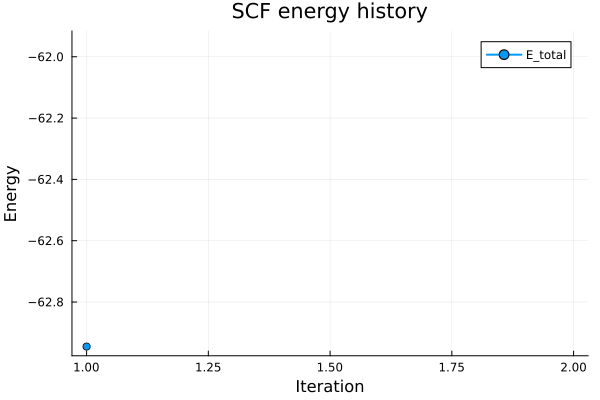
\includegraphics[width=\linewidth]{../../results_vault/experiment_08/U00/OBC/scf_energy.png}

\end{minipage}\hfill%
\begin{minipage}{0.49\linewidth}\centering

\textbf{PBC：収束}\par

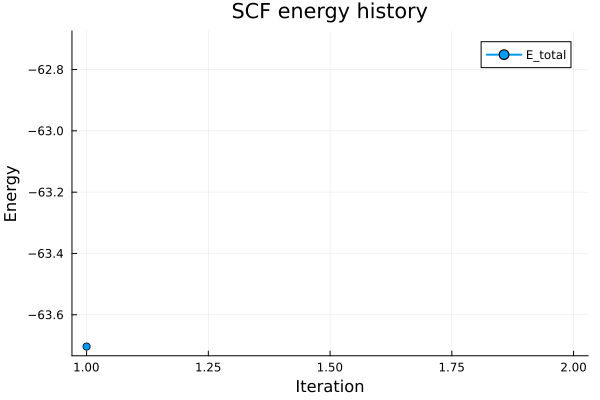
\includegraphics[width=\linewidth]{../../results_vault/experiment_08/U00/PBC/scf_energy.png}

\end{minipage}

\caption{U00。SCFエネルギーの比較。左：OBC、右：PBC。}\end{figure}

\begin{figure}[H]\centering

\begin{minipage}{0.49\linewidth}\centering

\textbf{OBC：収束}\par

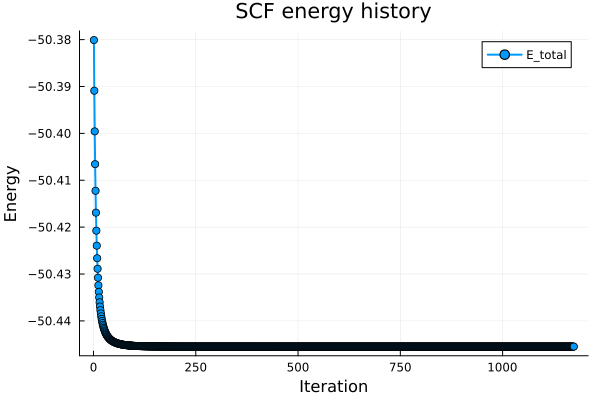
\includegraphics[width=\linewidth]{../../results_vault/experiment_08/U01/OBC/scf_energy.png}

\end{minipage}\hfill%
\begin{minipage}{0.49\linewidth}\centering

\textbf{PBC：収束}\par

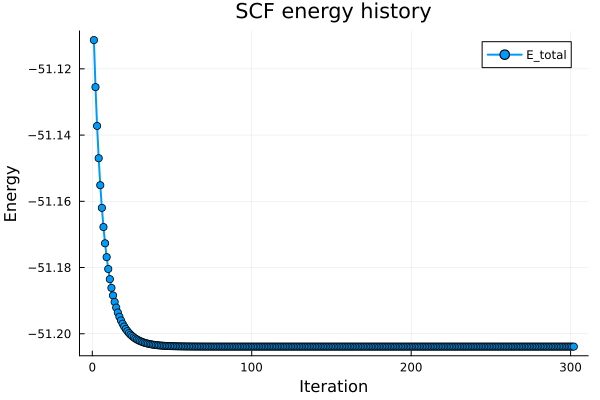
\includegraphics[width=\linewidth]{../../results_vault/experiment_08/U01/PBC/scf_energy.png}

\end{minipage}

\caption{U01。SCFエネルギーの比較。左：OBC、右：PBC。}\end{figure}

\begin{figure}[H]\centering

\begin{minipage}{0.49\linewidth}\centering

\textbf{OBC：収束}\par

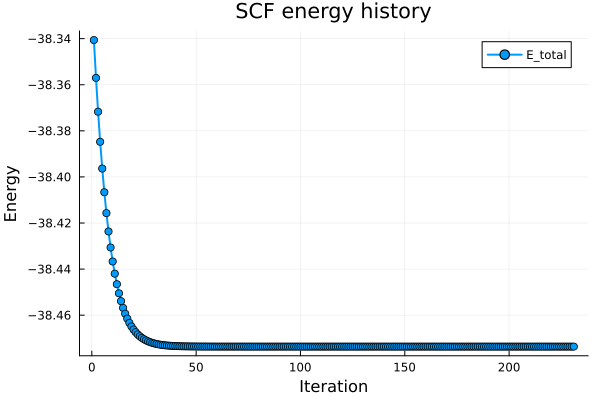
\includegraphics[width=\linewidth]{../../results_vault/experiment_08/U02/OBC/scf_energy.png}

\end{minipage}\hfill%
\begin{minipage}{0.49\linewidth}\centering

\textbf{PBC：収束}\par

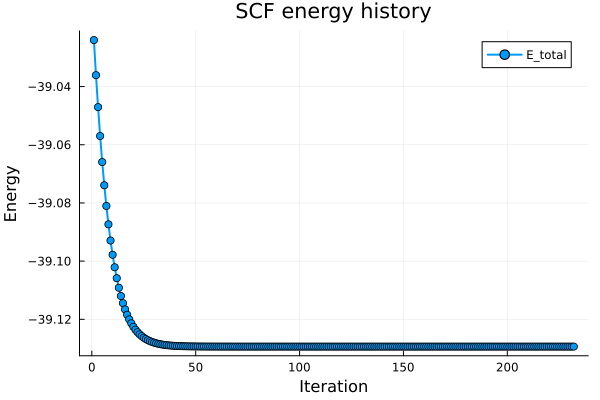
\includegraphics[width=\linewidth]{../../results_vault/experiment_08/U02/PBC/scf_energy.png}

\end{minipage}

\caption{U02。SCFエネルギーの比較。左：OBC、右：PBC。}\end{figure}

\begin{figure}[H]\centering

\begin{minipage}{0.49\linewidth}\centering

\textbf{OBC：収束}\par

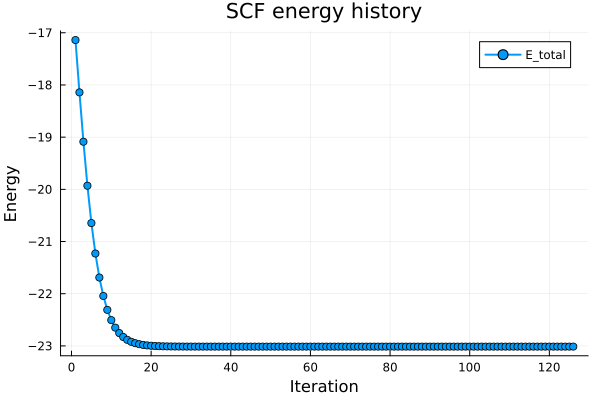
\includegraphics[width=\linewidth]{../../results_vault/experiment_08/U04/OBC/scf_energy.png}

\end{minipage}\hfill%
\begin{minipage}{0.49\linewidth}\centering

\textbf{PBC：収束}\par

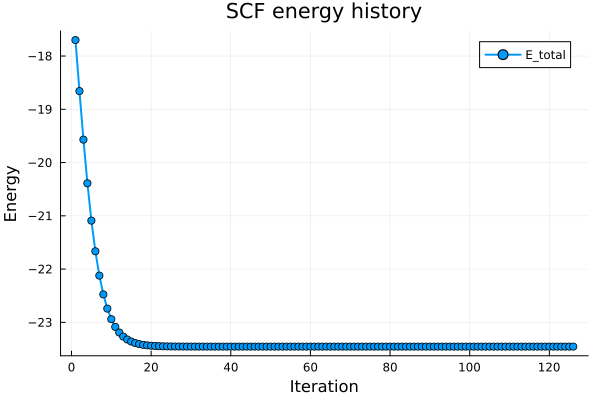
\includegraphics[width=\linewidth]{../../results_vault/experiment_08/U04/PBC/scf_energy.png}

\end{minipage}

\caption{U04。SCFエネルギーの比較。左：OBC、右：PBC。}\end{figure}

\begin{figure}[H]\centering

\begin{minipage}{0.49\linewidth}\centering

\textbf{OBC：収束}\par

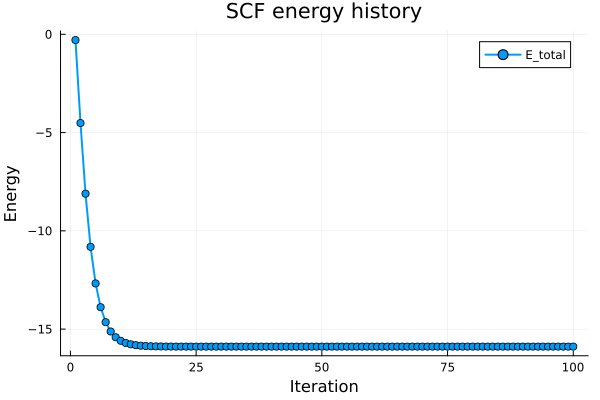
\includegraphics[width=\linewidth]{../../results_vault/experiment_08/U06/OBC/scf_energy.png}

\end{minipage}\hfill%
\begin{minipage}{0.49\linewidth}\centering

\textbf{PBC：収束}\par

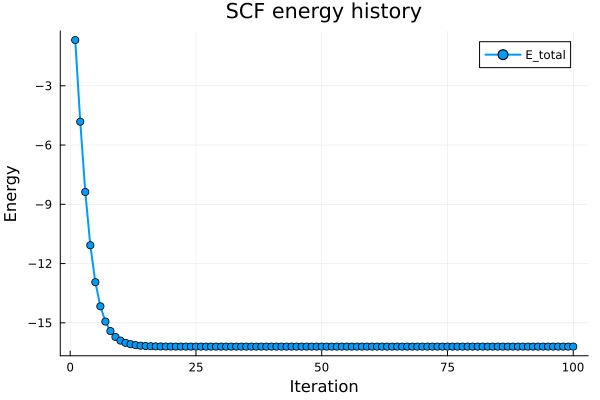
\includegraphics[width=\linewidth]{../../results_vault/experiment_08/U06/PBC/scf_energy.png}

\end{minipage}

\caption{U06。SCFエネルギーの比較。左：OBC、右：PBC。}\end{figure}

\begin{figure}[H]\centering

\begin{minipage}{0.49\linewidth}\centering

\textbf{OBC：収束}\par

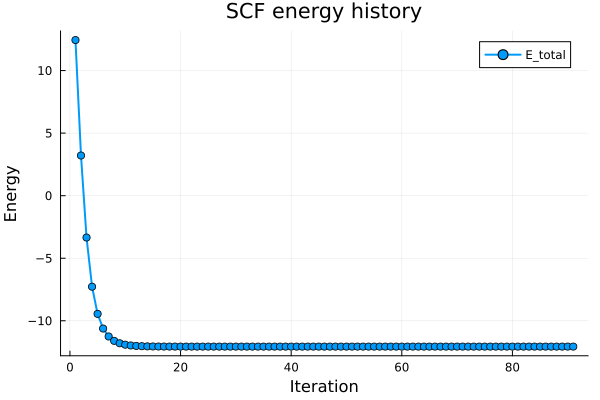
\includegraphics[width=\linewidth]{../../results_vault/experiment_08/U08/OBC/scf_energy.png}

\end{minipage}\hfill%
\begin{minipage}{0.49\linewidth}\centering

\textbf{PBC：収束}\par

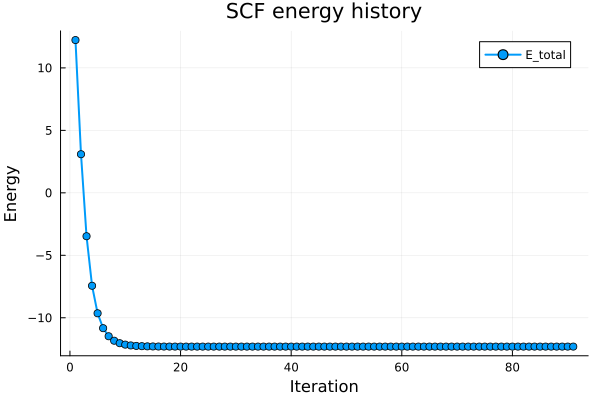
\includegraphics[width=\linewidth]{../../results_vault/experiment_08/U08/PBC/scf_energy.png}

\end{minipage}

\caption{U08。SCFエネルギーの比較。左：OBC、右：PBC。}\end{figure}

\chapter{SCF残差：自己無撞着性}

\sourcefile{scf_residual.png}

$U=1$ はOBCで1174反復、PBCで302反復を要し、最も遅い。$U=2$ では231・232、4では126、6では100、8では91反復となる。弱い相互作用で磁化が消えていく経路が特に遅い。一方 $U=0$ の1反復は初期状態がすでに固定点であり、この系列の収束速度の連続的な外挿には使えない。

残差は $r=\max_{i,\sigma}|F[n]_{i\sigma}-n_{i\sigma}|$。表は最終再評価値である。収束時には出力密度を採用してから再評価するため、履歴図の最後の残差とは同じとは限らない。

\begin{center}\small\setlength{\tabcolsep}{4pt}
\begin{longtable}{lrrr}
\toprule
条件/境界 & 状態 & 反復数 & 最終残差 \\ \midrule
\endhead
U00/OBC & 収束 & 1 & $0$ \\
U00/PBC & 収束 & 1 & $0$ \\
U01/OBC & 収束 & 1174 & $9.287\times10^{-11}$ \\
U01/PBC & 収束 & 302 & $7.282\times10^{-11}$ \\
U02/OBC & 収束 & 231 & $6.466\times10^{-11}$ \\
U02/PBC & 収束 & 232 & $6.429\times10^{-11}$ \\
U04/OBC & 収束 & 126 & $3.266\times10^{-11}$ \\
U04/PBC & 収束 & 126 & $3.263\times10^{-11}$ \\
U06/OBC & 収束 & 100 & $1.656\times10^{-11}$ \\
U06/PBC & 収束 & 100 & $1.651\times10^{-11}$ \\
U08/OBC & 収束 & 91 & $9.229\times10^{-12}$ \\
U08/PBC & 収束 & 91 & $9.162\times10^{-12}$ \\
\bottomrule\end{longtable}\end{center}

\begin{figure}[H]\centering

\begin{minipage}{0.49\linewidth}\centering

\textbf{OBC：収束}\par

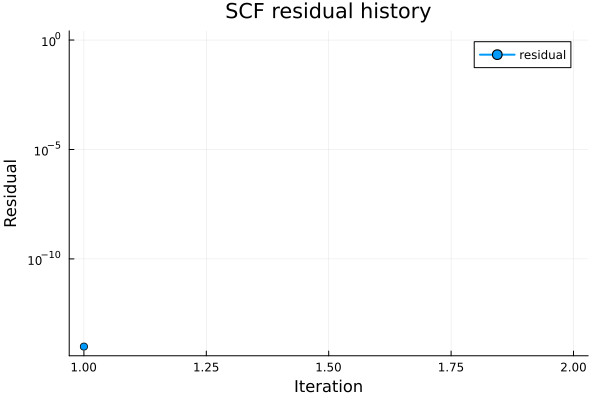
\includegraphics[width=\linewidth]{../../results_vault/experiment_08/U00/OBC/scf_residual.png}

\end{minipage}\hfill%
\begin{minipage}{0.49\linewidth}\centering

\textbf{PBC：収束}\par

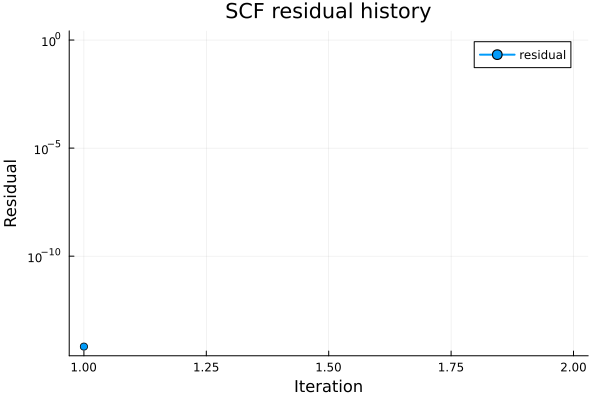
\includegraphics[width=\linewidth]{../../results_vault/experiment_08/U00/PBC/scf_residual.png}

\end{minipage}

\caption{U00。SCF残差の比較。左：OBC、右：PBC。}\end{figure}

\begin{figure}[H]\centering

\begin{minipage}{0.49\linewidth}\centering

\textbf{OBC：収束}\par

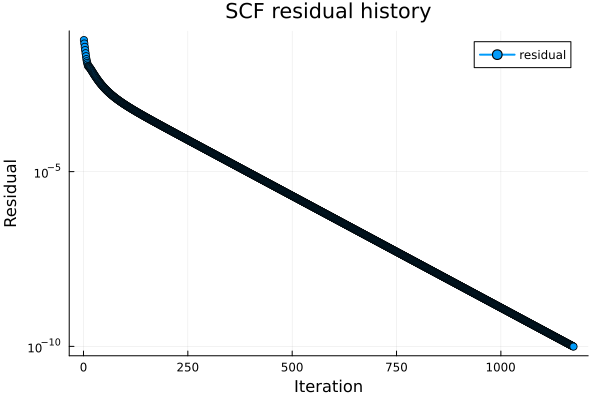
\includegraphics[width=\linewidth]{../../results_vault/experiment_08/U01/OBC/scf_residual.png}

\end{minipage}\hfill%
\begin{minipage}{0.49\linewidth}\centering

\textbf{PBC：収束}\par

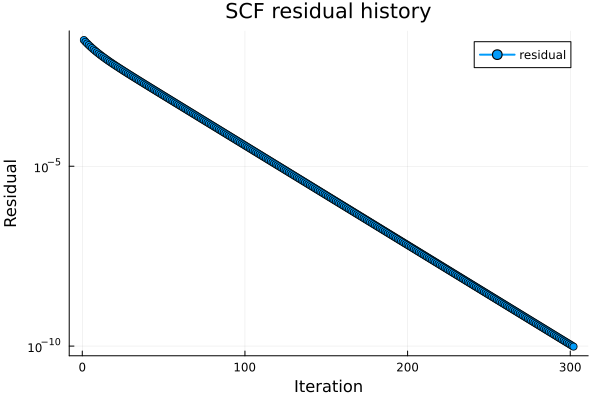
\includegraphics[width=\linewidth]{../../results_vault/experiment_08/U01/PBC/scf_residual.png}

\end{minipage}

\caption{U01。SCF残差の比較。左：OBC、右：PBC。}\end{figure}

\begin{figure}[H]\centering

\begin{minipage}{0.49\linewidth}\centering

\textbf{OBC：収束}\par

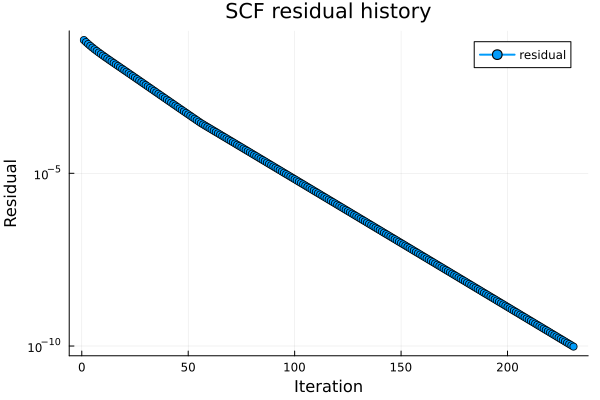
\includegraphics[width=\linewidth]{../../results_vault/experiment_08/U02/OBC/scf_residual.png}

\end{minipage}\hfill%
\begin{minipage}{0.49\linewidth}\centering

\textbf{PBC：収束}\par

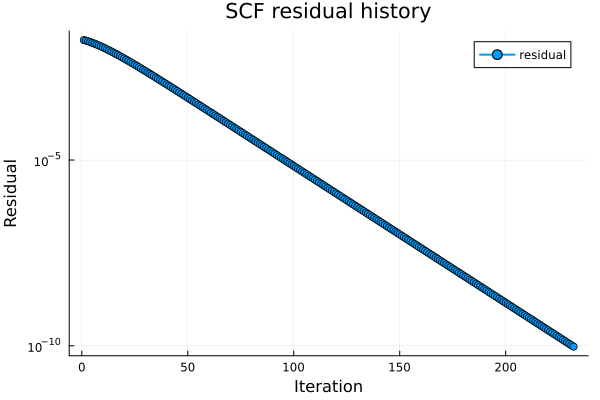
\includegraphics[width=\linewidth]{../../results_vault/experiment_08/U02/PBC/scf_residual.png}

\end{minipage}

\caption{U02。SCF残差の比較。左：OBC、右：PBC。}\end{figure}

\begin{figure}[H]\centering

\begin{minipage}{0.49\linewidth}\centering

\textbf{OBC：収束}\par

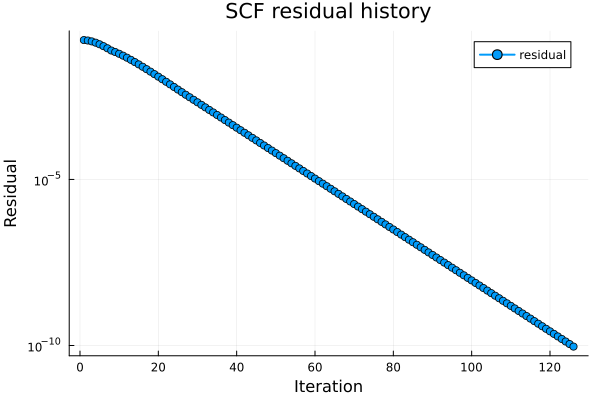
\includegraphics[width=\linewidth]{../../results_vault/experiment_08/U04/OBC/scf_residual.png}

\end{minipage}\hfill%
\begin{minipage}{0.49\linewidth}\centering

\textbf{PBC：収束}\par

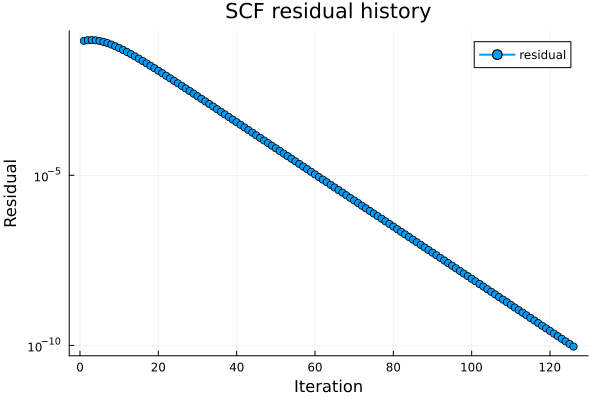
\includegraphics[width=\linewidth]{../../results_vault/experiment_08/U04/PBC/scf_residual.png}

\end{minipage}

\caption{U04。SCF残差の比較。左：OBC、右：PBC。}\end{figure}

\begin{figure}[H]\centering

\begin{minipage}{0.49\linewidth}\centering

\textbf{OBC：収束}\par

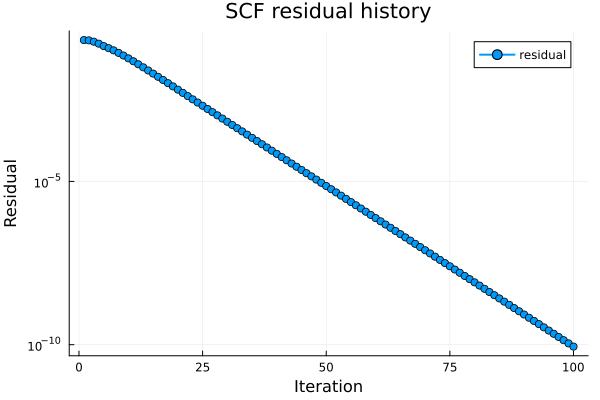
\includegraphics[width=\linewidth]{../../results_vault/experiment_08/U06/OBC/scf_residual.png}

\end{minipage}\hfill%
\begin{minipage}{0.49\linewidth}\centering

\textbf{PBC：収束}\par

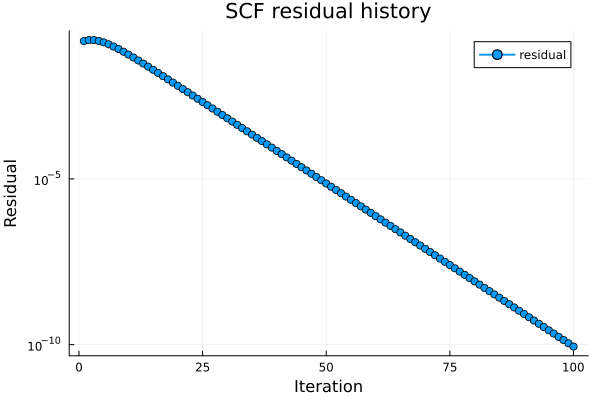
\includegraphics[width=\linewidth]{../../results_vault/experiment_08/U06/PBC/scf_residual.png}

\end{minipage}

\caption{U06。SCF残差の比較。左：OBC、右：PBC。}\end{figure}

\begin{figure}[H]\centering

\begin{minipage}{0.49\linewidth}\centering

\textbf{OBC：収束}\par

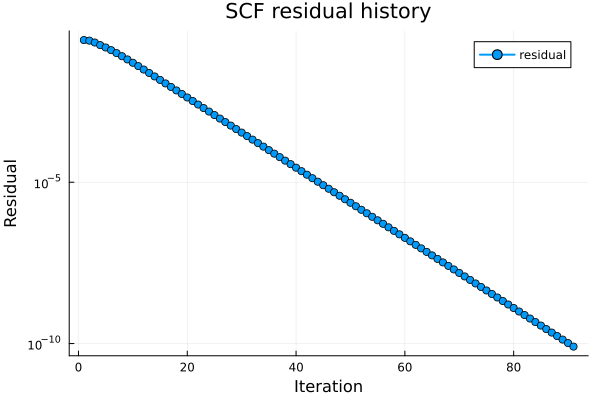
\includegraphics[width=\linewidth]{../../results_vault/experiment_08/U08/OBC/scf_residual.png}

\end{minipage}\hfill%
\begin{minipage}{0.49\linewidth}\centering

\textbf{PBC：収束}\par

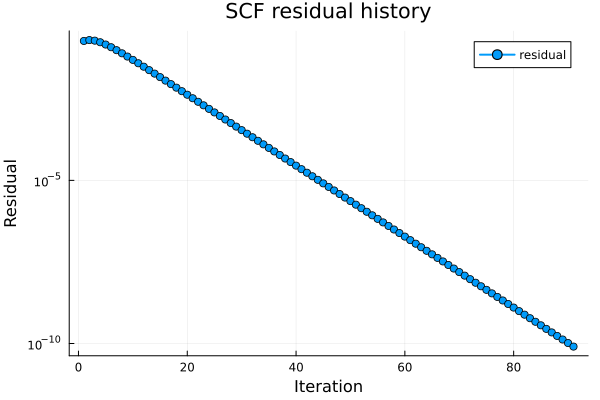
\includegraphics[width=\linewidth]{../../results_vault/experiment_08/U08/PBC/scf_residual.png}

\end{minipage}

\caption{U08。SCF残差の比較。左：OBC、右：PBC。}\end{figure}

\chapter{軌道エネルギー：準位構造}

\sourcefile{final_orbital_energies.png}

$U=0,1$ では非相互作用に近い準位列が見られ、$U\ge2$ では中央の分離が増大する。平均場の中心は概ね $U/2$ へ移動するため、単なる縦方向のシフトと占有・非占有準位の分離を区別する。$U=0$ でも有限サイズの準位間隔があるので、図の空白をすべて相互作用ギャップと呼ぶべきではない。

横軸はエネルギー昇順の軌道番号、縦軸は $h_\sigma=h_0+U\operatorname{diag}(n_{\bar\sigma})$ の固有値である。固有値の数値ファイルは保存されていないため、図からの解釈は定性的なものに留める。未収束例をCSVから再対角化すると保存図とは異なる平均場になる可能性があり、本書ではその置換を行わない。

\begin{figure}[H]\centering

\begin{minipage}{0.49\linewidth}\centering

\textbf{OBC：収束}\par

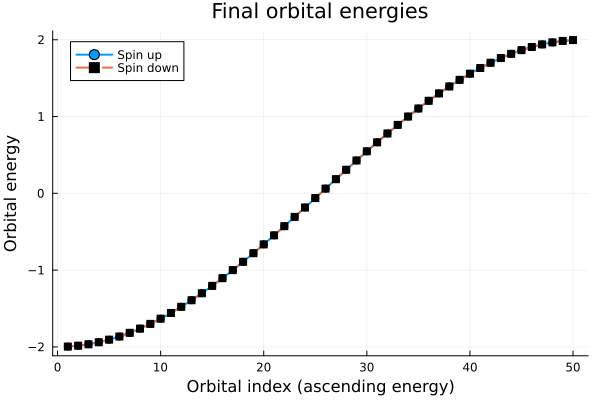
\includegraphics[width=\linewidth]{../../results_vault/experiment_08/U00/OBC/final_orbital_energies.png}

\end{minipage}\hfill%
\begin{minipage}{0.49\linewidth}\centering

\textbf{PBC：収束}\par

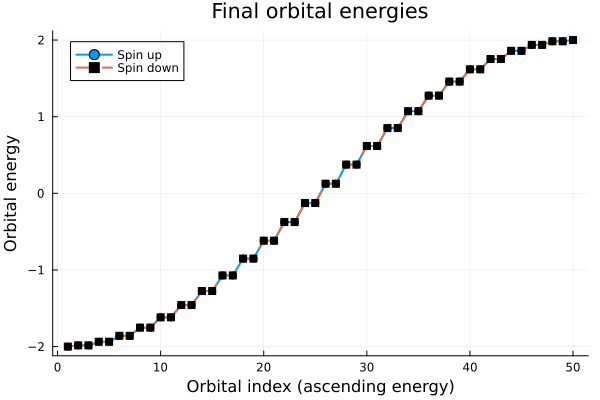
\includegraphics[width=\linewidth]{../../results_vault/experiment_08/U00/PBC/final_orbital_energies.png}

\end{minipage}

\caption{U00。軌道エネルギーの比較。左：OBC、右：PBC。}\end{figure}

\begin{figure}[H]\centering

\begin{minipage}{0.49\linewidth}\centering

\textbf{OBC：収束}\par

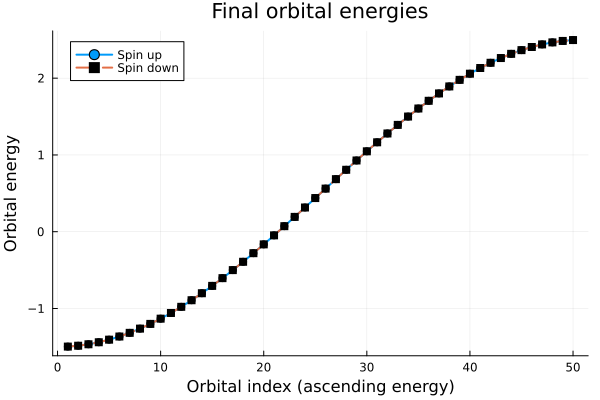
\includegraphics[width=\linewidth]{../../results_vault/experiment_08/U01/OBC/final_orbital_energies.png}

\end{minipage}\hfill%
\begin{minipage}{0.49\linewidth}\centering

\textbf{PBC：収束}\par

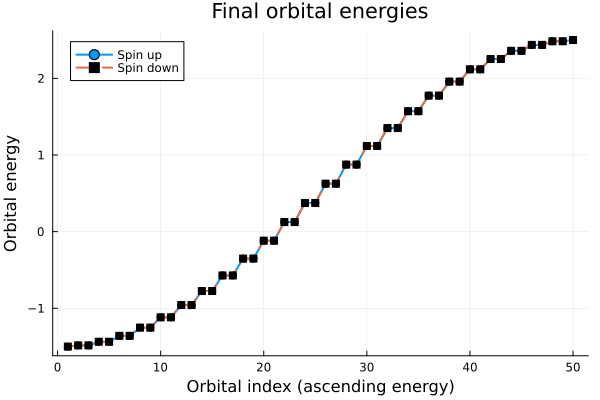
\includegraphics[width=\linewidth]{../../results_vault/experiment_08/U01/PBC/final_orbital_energies.png}

\end{minipage}

\caption{U01。軌道エネルギーの比較。左：OBC、右：PBC。}\end{figure}

\begin{figure}[H]\centering

\begin{minipage}{0.49\linewidth}\centering

\textbf{OBC：収束}\par

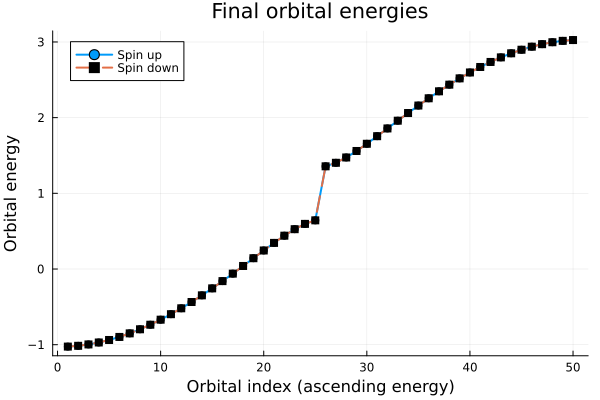
\includegraphics[width=\linewidth]{../../results_vault/experiment_08/U02/OBC/final_orbital_energies.png}

\end{minipage}\hfill%
\begin{minipage}{0.49\linewidth}\centering

\textbf{PBC：収束}\par

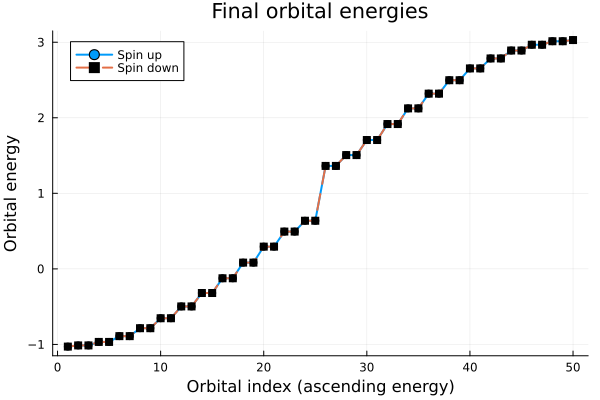
\includegraphics[width=\linewidth]{../../results_vault/experiment_08/U02/PBC/final_orbital_energies.png}

\end{minipage}

\caption{U02。軌道エネルギーの比較。左：OBC、右：PBC。}\end{figure}

\begin{figure}[H]\centering

\begin{minipage}{0.49\linewidth}\centering

\textbf{OBC：収束}\par

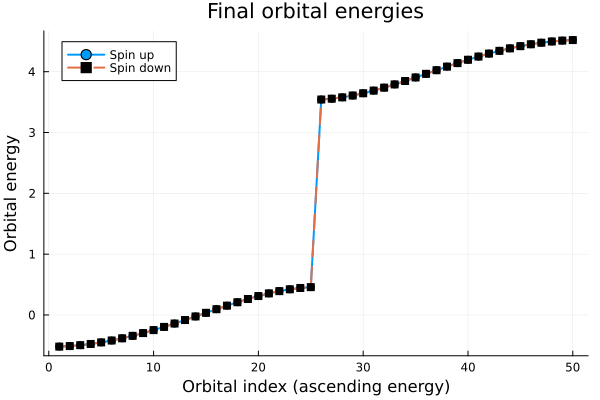
\includegraphics[width=\linewidth]{../../results_vault/experiment_08/U04/OBC/final_orbital_energies.png}

\end{minipage}\hfill%
\begin{minipage}{0.49\linewidth}\centering

\textbf{PBC：収束}\par

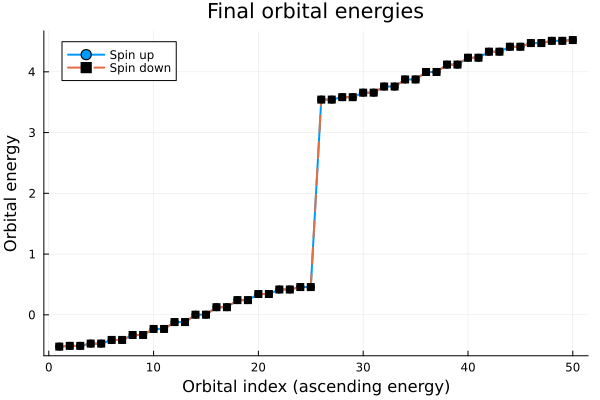
\includegraphics[width=\linewidth]{../../results_vault/experiment_08/U04/PBC/final_orbital_energies.png}

\end{minipage}

\caption{U04。軌道エネルギーの比較。左：OBC、右：PBC。}\end{figure}

\begin{figure}[H]\centering

\begin{minipage}{0.49\linewidth}\centering

\textbf{OBC：収束}\par

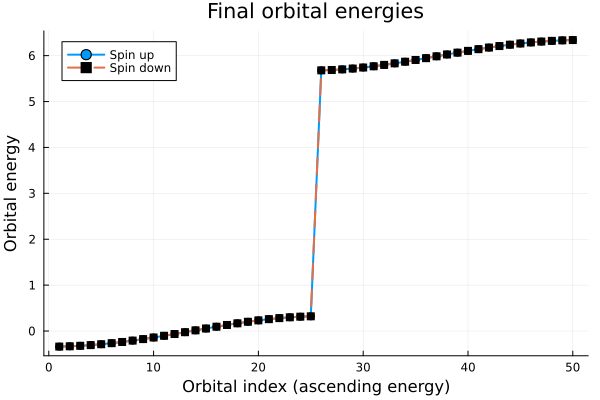
\includegraphics[width=\linewidth]{../../results_vault/experiment_08/U06/OBC/final_orbital_energies.png}

\end{minipage}\hfill%
\begin{minipage}{0.49\linewidth}\centering

\textbf{PBC：収束}\par

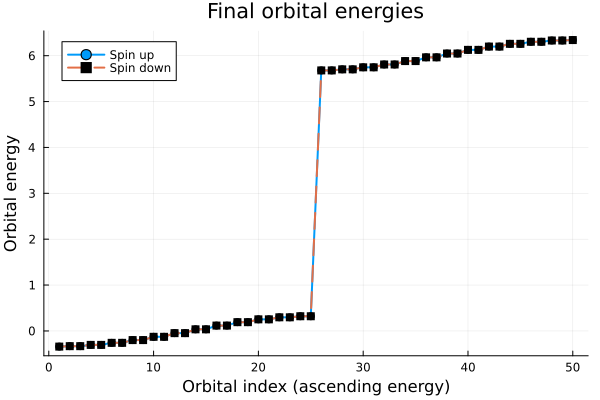
\includegraphics[width=\linewidth]{../../results_vault/experiment_08/U06/PBC/final_orbital_energies.png}

\end{minipage}

\caption{U06。軌道エネルギーの比較。左：OBC、右：PBC。}\end{figure}

\begin{figure}[H]\centering

\begin{minipage}{0.49\linewidth}\centering

\textbf{OBC：収束}\par

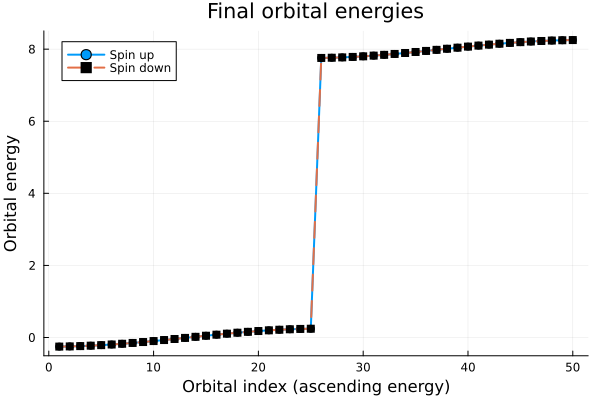
\includegraphics[width=\linewidth]{../../results_vault/experiment_08/U08/OBC/final_orbital_energies.png}

\end{minipage}\hfill%
\begin{minipage}{0.49\linewidth}\centering

\textbf{PBC：収束}\par

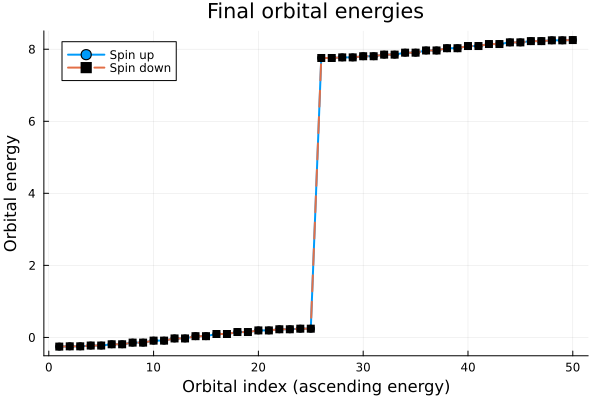
\includegraphics[width=\linewidth]{../../results_vault/experiment_08/U08/PBC/final_orbital_energies.png}

\end{minipage}

\caption{U08。軌道エネルギーの比較。左：OBC、右：PBC。}\end{figure}

\chapter{局所磁化：空間構造}

\sourcefile{final_magnetization.png}

PBCの $\overline{|m|}$ は $U=2,4,6,8$ で0.340372、0.768964、0.892299、0.938536と増大する。OBCは端でより強い磁化を持つ。$U=1$ の最大磁化はOBCで約 $2.99\times10^{-9}$、PBCで約 $4.44\times10^{-10}$ にすぎない。自動縮尺の図では大きく振動して見えるが、有限振幅の反強磁性と同列には扱わない。

$\overline{|m|}=L^{-1}\sum_i|m_i|$、$M_{\rm AF}=|L^{-1}\sum_i(-1)^im_i|$ と定義する。$m_i$ はスピン密度差であり、$\langle S_i^z\rangle=m_i/2$ に対応する。全磁化は $\sum_i m_i=\Delta N$ と粒子数制約で固定される。

\begin{center}\small\setlength{\tabcolsep}{4pt}
\begin{longtable}{lrrr}
\toprule
条件/境界 & 状態 & $\overline{|m|}$ & $M_{\rm AF}$ \\ \midrule
\endhead
U00/OBC & 収束 & 0.000000 & 0.000000 \\
U00/PBC & 収束 & 0.000000 & 0.000000 \\
U01/OBC & 収束 & 0.000000 & 0.000000 \\
U01/PBC & 収束 & 0.000000 & 0.000000 \\
U02/OBC & 収束 & 0.350854 & 0.350854 \\
U02/PBC & 収束 & 0.340372 & 0.340372 \\
U04/OBC & 収束 & 0.773051 & 0.773051 \\
U04/PBC & 収束 & 0.768964 & 0.768964 \\
U06/OBC & 収束 & 0.894335 & 0.894335 \\
U06/PBC & 収束 & 0.892299 & 0.892299 \\
U08/OBC & 収束 & 0.939727 & 0.939727 \\
U08/PBC & 収束 & 0.938536 & 0.938536 \\
\bottomrule\end{longtable}\end{center}

\begin{figure}[H]\centering

\begin{minipage}{0.49\linewidth}\centering

\textbf{OBC：収束}\par

\includegraphics[width=\linewidth]{../../results_vault/experiment_08/U00/OBC/final_magnetization.png}

\end{minipage}\hfill%
\begin{minipage}{0.49\linewidth}\centering

\textbf{PBC：収束}\par

\includegraphics[width=\linewidth]{../../results_vault/experiment_08/U00/PBC/final_magnetization.png}

\end{minipage}

\caption{U00。局所磁化の比較。左：OBC、右：PBC。}\end{figure}

\begin{figure}[H]\centering

\begin{minipage}{0.49\linewidth}\centering

\textbf{OBC：収束}\par

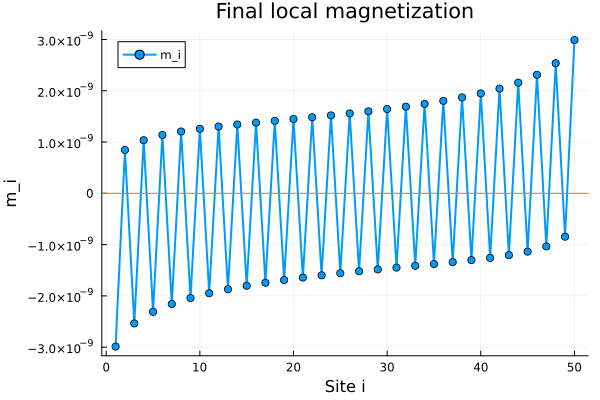
\includegraphics[width=\linewidth]{../../results_vault/experiment_08/U01/OBC/final_magnetization.png}

\end{minipage}\hfill%
\begin{minipage}{0.49\linewidth}\centering

\textbf{PBC：収束}\par

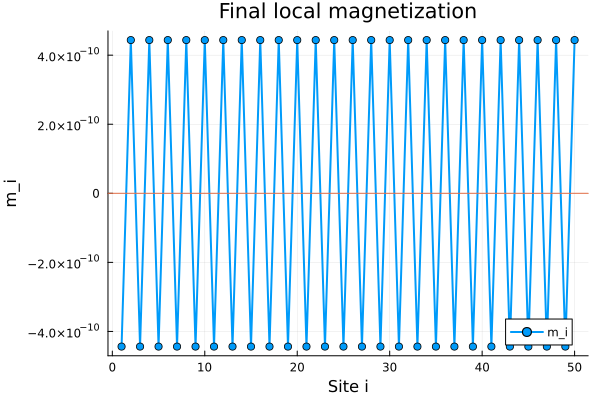
\includegraphics[width=\linewidth]{../../results_vault/experiment_08/U01/PBC/final_magnetization.png}

\end{minipage}

\caption{U01。局所磁化の比較。左：OBC、右：PBC。}\end{figure}

\begin{figure}[H]\centering

\begin{minipage}{0.49\linewidth}\centering

\textbf{OBC：収束}\par

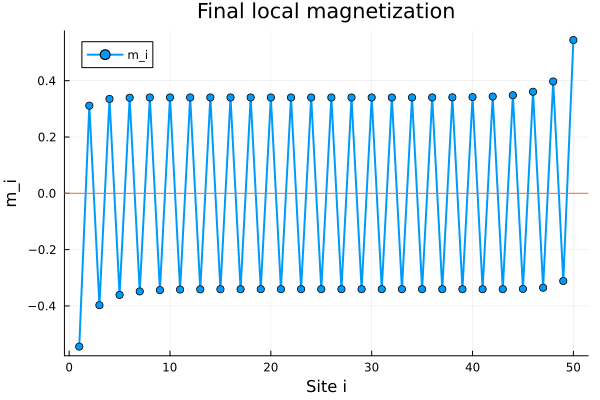
\includegraphics[width=\linewidth]{../../results_vault/experiment_08/U02/OBC/final_magnetization.png}

\end{minipage}\hfill%
\begin{minipage}{0.49\linewidth}\centering

\textbf{PBC：収束}\par

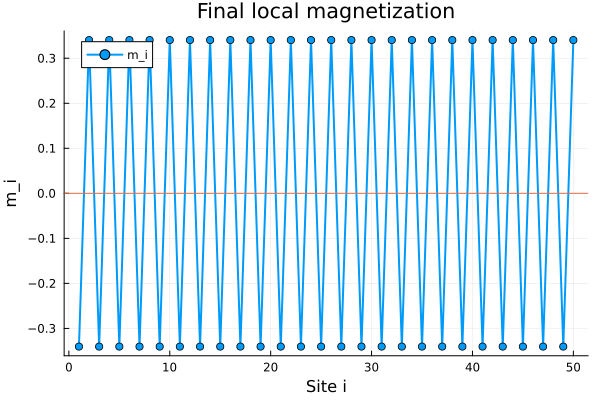
\includegraphics[width=\linewidth]{../../results_vault/experiment_08/U02/PBC/final_magnetization.png}

\end{minipage}

\caption{U02。局所磁化の比較。左：OBC、右：PBC。}\end{figure}

\begin{figure}[H]\centering

\begin{minipage}{0.49\linewidth}\centering

\textbf{OBC：収束}\par

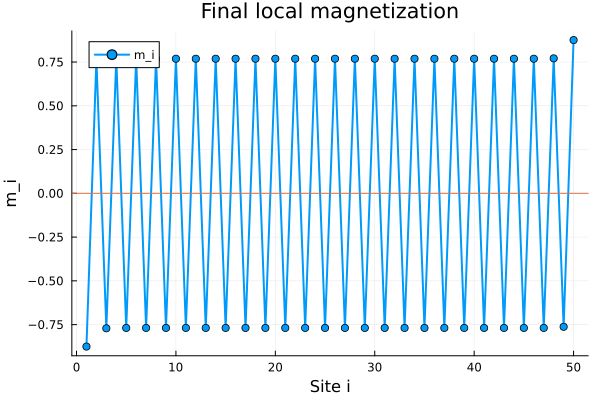
\includegraphics[width=\linewidth]{../../results_vault/experiment_08/U04/OBC/final_magnetization.png}

\end{minipage}\hfill%
\begin{minipage}{0.49\linewidth}\centering

\textbf{PBC：収束}\par

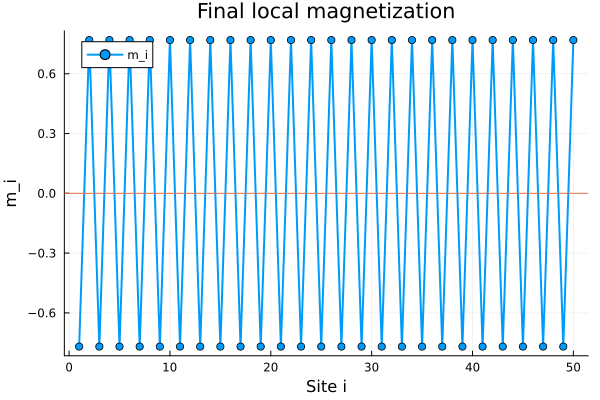
\includegraphics[width=\linewidth]{../../results_vault/experiment_08/U04/PBC/final_magnetization.png}

\end{minipage}

\caption{U04。局所磁化の比較。左：OBC、右：PBC。}\end{figure}

\begin{figure}[H]\centering

\begin{minipage}{0.49\linewidth}\centering

\textbf{OBC：収束}\par

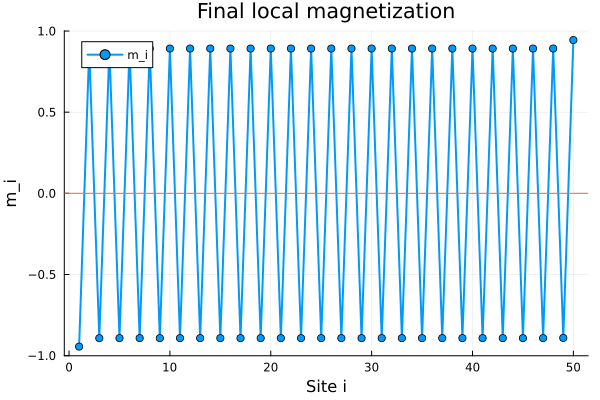
\includegraphics[width=\linewidth]{../../results_vault/experiment_08/U06/OBC/final_magnetization.png}

\end{minipage}\hfill%
\begin{minipage}{0.49\linewidth}\centering

\textbf{PBC：収束}\par

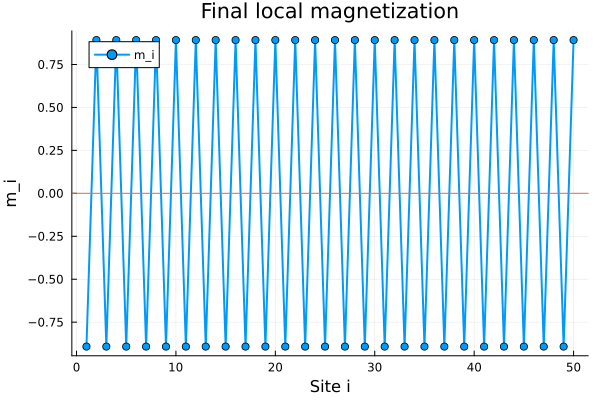
\includegraphics[width=\linewidth]{../../results_vault/experiment_08/U06/PBC/final_magnetization.png}

\end{minipage}

\caption{U06。局所磁化の比較。左：OBC、右：PBC。}\end{figure}

\begin{figure}[H]\centering

\begin{minipage}{0.49\linewidth}\centering

\textbf{OBC：収束}\par

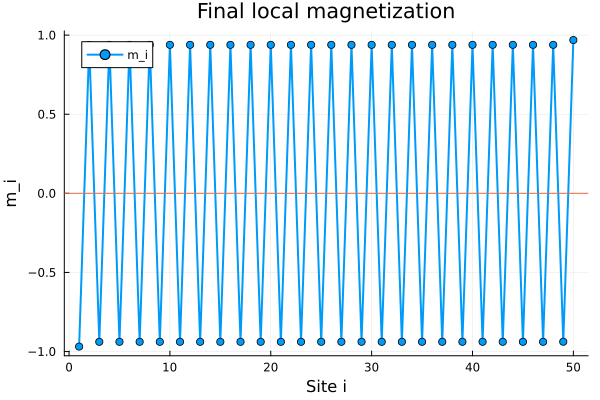
\includegraphics[width=\linewidth]{../../results_vault/experiment_08/U08/OBC/final_magnetization.png}

\end{minipage}\hfill%
\begin{minipage}{0.49\linewidth}\centering

\textbf{PBC：収束}\par

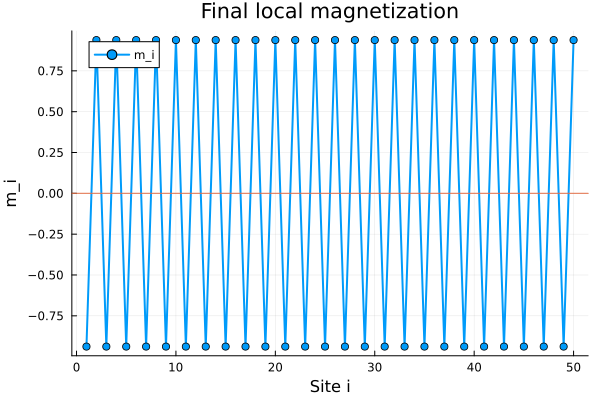
\includegraphics[width=\linewidth]{../../results_vault/experiment_08/U08/PBC/final_magnetization.png}

\end{minipage}

\caption{U08。局所磁化の比較。左：OBC、右：PBC。}\end{figure}

\chapter{境界条件による全エネルギー差}

\sourcefile{boundary_energy_difference.png}

$\Delta E_{\rm boundary}=E_{\rm PBC}-E_{\rm OBC}$ と定義する。負ならPBC、正ならOBCの保存された解の方が低エネルギーである。両方が収束した組だけを表と図で数値比較し、それ以外をNCとする。

境界差は $U=0,1$ で約 $-0.758400$、2で $-0.655736$、4で $-0.442191$、6で $-0.315382$、8で $-0.242317$ となり、強相互作用側で絶対値が小さくなる。$U=1$ で0と同じ差になるのは、ほぼ一様な密度に対する相互作用項が両境界で同じだけ加わるためである。強結合側の減少はホッピングによるエネルギー利得の縮小と整合するが、$U$ やサイズの漸近則をこの6点だけで確定しない。

\begin{center}\small\setlength{\tabcolsep}{4pt}
\begin{longtable}{lrr}
\toprule
条件 & $\Delta E_{\rm boundary}$ & $\Delta E_{\rm boundary}/L$ \\ \midrule
\endhead
U00 & -0.758399879117 & -0.015167997582 \\
U01 & -0.758399879117 & -0.015167997582 \\
U02 & -0.655736385778 & -0.013114727716 \\
U04 & -0.442191290827 & -0.008843825817 \\
U06 & -0.315381890677 & -0.006307637814 \\
U08 & -0.242316879209 & -0.004846337584 \\
\bottomrule\end{longtable}\end{center}

\begin{figure}[H]\centering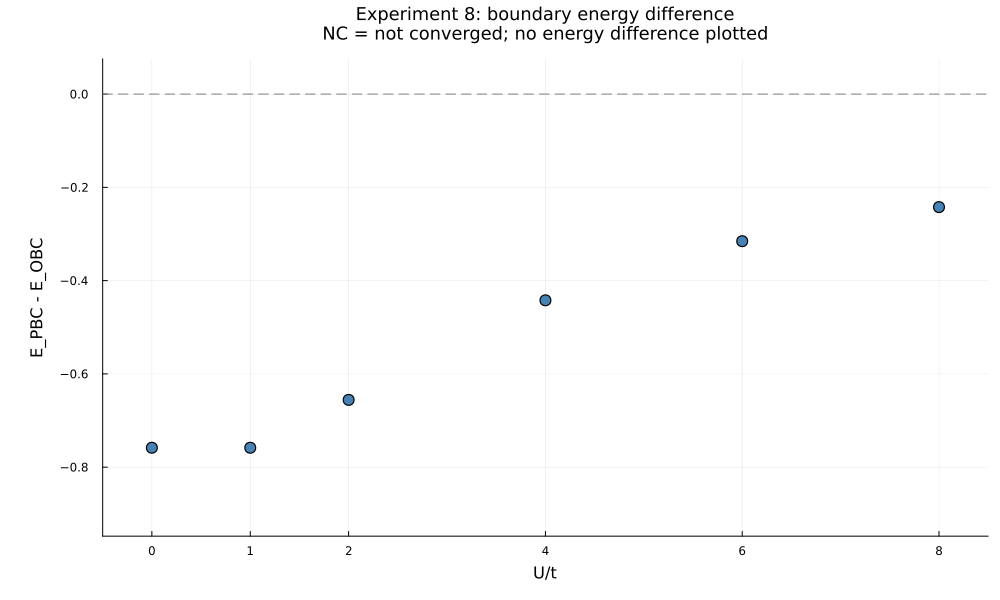
\includegraphics[width=0.9\linewidth]{../../results_vault/experiment_08/boundary_energy_difference.png}\caption{保存済みの境界エネルギー差。NCは未収束の組を示し、差が0であることを意味しない。}\end{figure}

\section*{結論と残された確認}

半充填・非偏極で $U/t=0,1,2,4,6,8$ を比較した。全12ケースが収束する。$U=0$ のみ一様型初期密度を再利用し、それ以外は反強磁性型から開始した。$U=1$ では初期磁化がほぼ消え、$U\ge2$ では大きな交互磁化が残る。ただし有限サイズの離散的な掃引から臨界値や厳密系の相転移を決定することはできない。

対象ケースはすべて収束した。ただし、収束判定だけでは得られた解が大域的な最小エネルギー状態であることまでは保証されない。

サイズは50に固定しているため、境界効果と有限サイズ効果の切り分けには別サイズの結果が必要である。

\end{document}